\documentclass[DIV=15]{scrartcl}

\usepackage{tikz}
\usetikzlibrary{arrows.meta}

\begin{document}

\section*{Aufgabe 1}

Berechne die Länge $x$.\\

\resizebox{0.7\textwidth}{!}{%
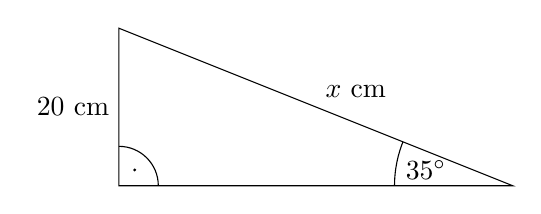
\begin{tikzpicture}
    \draw (0, 0) -- (5, 0) -- (0, 2)
	node [midway, above right] {$x$ cm} -- cycle
	node [midway, left] {20 cm};
    \path[clip] (0, 0) -- (5, 0) -- (0, 2) -- cycle;
    \draw (5, 0) circle (1.5);
    \node at (3.9, 0.2) {$35^\circ$};
    \draw (0.5, 0) arc (0:90:0.5);
    \draw[fill=black] (0.2, 0.2) circle (0.01);
\end{tikzpicture}
}

\section*{Aufgabe 2}

Berechne die Länge $x$.\\

\resizebox{0.7\textwidth}{!}{%
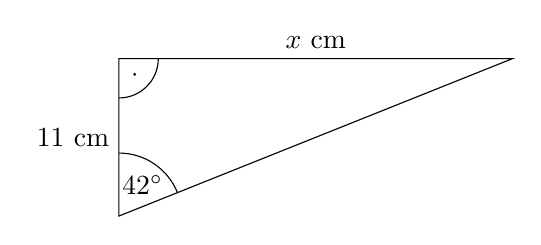
\begin{tikzpicture}
    \draw (0, 0) -- (0, -2)
	node [midway, left] {11 cm} -- (5, 0)
	-- cycle node [midway, above] {$x$ cm};
    \path[clip] (0, 0) -- (0, -2) -- (5, 0) -- cycle;
    \draw (0, -2) circle (0.8);
    \node at (0.3, -1.6) {$42^\circ$};
    \draw (0.5, 0) arc (0:-90:0.5);
    \draw[fill=black] (0.2, -0.2) circle (0.01);
\end{tikzpicture}
}

\section*{Aufgabe 3}

Berechne den Winkel $x$.\\

\resizebox{0.6\textwidth}{!}{%
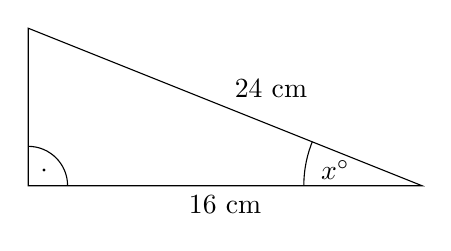
\begin{tikzpicture}
    \draw (0, 0) -- (5, 0)
	node [midway, below] {16 cm} -- (0, 2)
	node [midway, above right] {24 cm} -- cycle;
    \path[clip] (0, 0) -- (5, 0) -- (0, 2) -- cycle;
    \draw (5, 0) circle (1.5);
    \node at (3.9, 0.2) {$x^\circ$};
    \draw (0.5, 0) arc (0:90:0.5);
    \draw[fill=black] (0.2, 0.2) circle (0.01);
\end{tikzpicture}
}

\newpage

\section*{Aufgabe 4}

Berechne den Winkel $x$.\\

\resizebox{0.7\textwidth}{!}{%
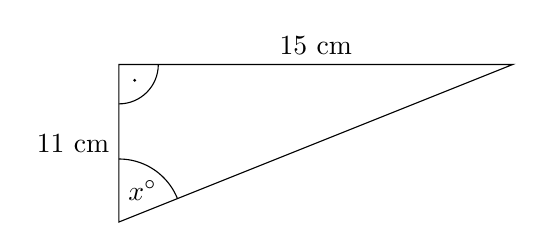
\begin{tikzpicture}
    \draw (0, 0) -- (0, -2)
	node [midway, left] {11 cm} -- (5, 0)
	-- cycle node [midway, above] {15 cm};
    \path[clip] (0, 0) -- (0, -2) -- (5, 0) -- cycle;
    \draw (0, -2) circle (0.8);
    \node at (0.3, -1.6) {$x^\circ$};
    \draw (0.5, 0) arc (0:-90:0.5);
    \draw[fill=black] (0.2, -0.2) circle (0.01);
\end{tikzpicture}
}

\section*{Aufgabe 5}

Berechne die Länge $AB$.\\

\resizebox{0.7\textwidth}{!}{%
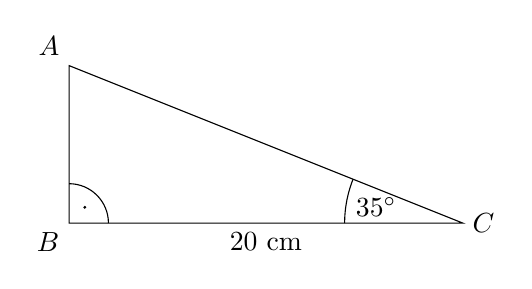
\begin{tikzpicture}
    \draw (0, 0)
	node [below left] {$B$} -- (5, 0)
        node [right] {$C$}
	node [midway, below] {20 cm} -- (0, 2)
	node [above left] {$A$} -- cycle;
    \path[clip] (0, 0) -- (5, 0) -- (0, 2) -- cycle;
    \draw (5, 0) circle (1.5);
    \node at (3.9, 0.2) {$35^\circ$};
    \draw (0.5, 0) arc (0:90:0.5);
    \draw[fill=black] (0.2, 0.2) circle (0.01);
\end{tikzpicture}
}

\section*{Aufgabe 6}

Berechne die Länge $AB$.\\

\resizebox{0.6\textwidth}{!}{%
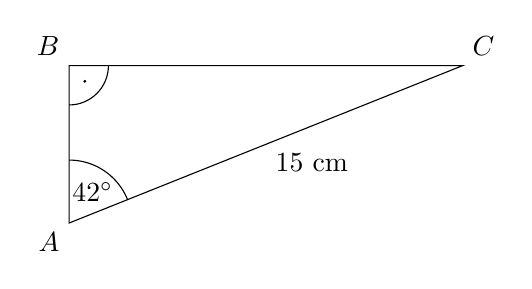
\begin{tikzpicture}
    \draw (0, 0)
	node [above left] {$B$} -- (0, -2)
	node [below left] {$A$} -- (5, 0)
	node [above right] {$C$}
	node [midway, below right] {15 cm} -- cycle;
    \path[clip] (0, 0) -- (0, -2) -- (5, 0) -- cycle;
    \draw (0, -2) circle (0.8);
    \node at (0.3, -1.6) {$42^\circ$};
    \draw (0.5, 0) arc (0:-90:0.5);
    \draw[fill=black] (0.2, -0.2) circle (0.01);
\end{tikzpicture}
}

\section*{Aufgabe 7}

Berechne den Winkel $ACB$.\\

\resizebox{0.7\textwidth}{!}{%
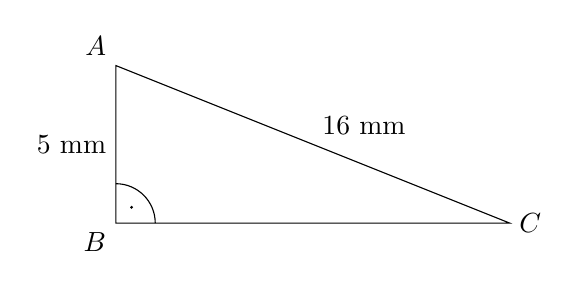
\begin{tikzpicture}
    \draw (0, 0)
	node [below left] {$B$} -- (5, 0)
        node [right] {$C$} -- (0, 2)
	node [midway, above right] {16 mm}
	node [above left] {$A$} -- cycle
	node [midway, left] {5 mm};
    \draw (0.5, 0) arc (0:90:0.5);
    \draw[fill=black] (0.2, 0.2) circle (0.01);
\end{tikzpicture}
}

\section*{Aufgabe 8}

Berechne den Winkel $BAC$.\\

\resizebox{0.7\textwidth}{!}{%
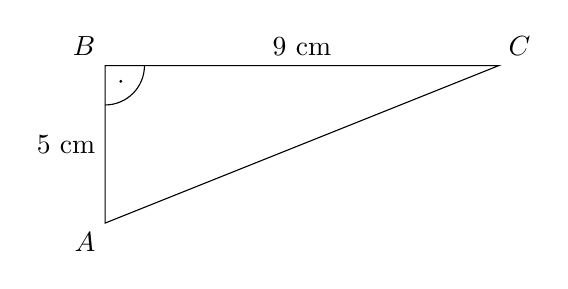
\begin{tikzpicture}
    \draw (0, 0)
	node [above left] {$B$} -- (0, -2)
	node [midway, left] {5 cm}
	node [below left] {$A$} -- (5, 0)
	node [above right] {$C$}
	-- cycle
	node [midway, above] {9 cm};
    \path[clip] (0, 0) -- (0, -2) -- (5, 0) -- cycle;
    \draw (0.5, 0) arc (0:-90:0.5);
    \draw[fill=black] (0.2, -0.2) circle (0.01);
\end{tikzpicture}
}

\section*{Aufgabe 9}

Berechne den Winkel $BAD$.\\

\resizebox{0.6\textwidth}{!}{%
\begin{tikzpicture}
    \draw (0, 0)
	node [below left] {$A$} -- (0, -2)
	node [midway, left] {4 m}
	node [below left] {$B$} -- (6, -2)
	node [below right] {$C$}
	node [midway, below] {15 m} -- (6, 1.5)
	node [above right] {$D$}
	node [midway, right] {6 m} -- cycle;

    \draw (0.5, -2) arc (0:90:0.5);
    \draw[fill=black] (0.2, -1.8) circle (0.01);

    \draw (6, -1.5) arc (90:180:0.5);
    \draw[fill=black] (5.8, -1.8) circle (0.01);
\end{tikzpicture}
}

\section*{Aufgabe 10}

Berechne die Länge $x$.\\

\resizebox{0.7\textwidth}{!}{%
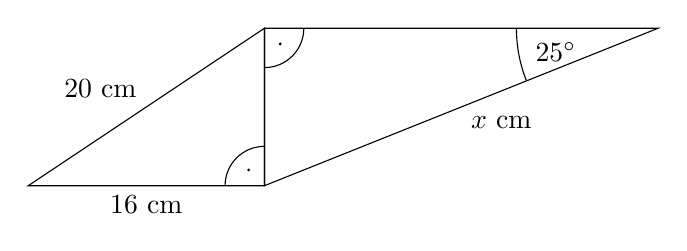
\begin{tikzpicture}
    \draw (0, 0) -- (3, 0)
	node [midway, below] {16 cm} -- (3, 2) -- cycle
	node [midway, above left] {20 cm};
    \draw (3, 0) -- (8, 2)
	node [midway, below right] {$x$ cm} -- (3, 2) -- cycle;
    \draw (3, 0.5) arc (90:180:0.5);
    \draw[fill=black] (2.8, 0.2) circle (0.01);

    \draw (3.5, 2) arc (0:-90:0.5);
    \draw[fill=black] (3.2, 1.8) circle (0.01);

    \path[clip] (3, 0) -- (8, 2)  -- (3, 2) -- cycle;
    \draw (8, 2) circle (1.8);
    \node at (6.7, 1.7) {$25^\circ$};
\end{tikzpicture}
}

\section*{Aufgabe 11}

Berechne den Winkel $BCD$.\\

\resizebox{0.7\textwidth}{!}{%
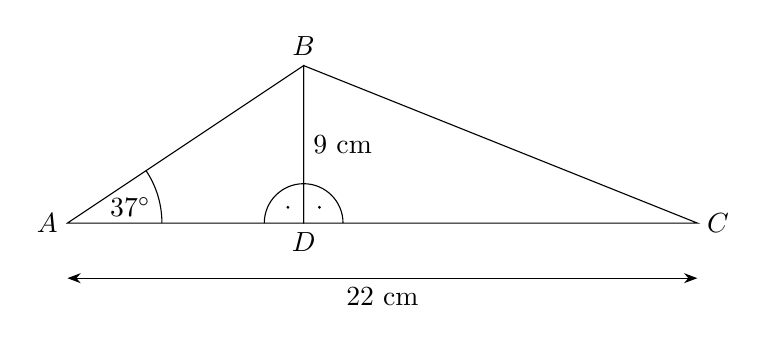
\begin{tikzpicture}
    \draw (0, 0)
	node [left] {$A$} -- (3, 0)
	node [below] {$D$} -- (3, 2)
	node [above] {$B$}
	node [midway, right] {9 cm} -- cycle;
    \draw (3, 0.5) arc (90:180:0.5);
    \draw[fill=black] (2.8, 0.2) circle (0.01);

    \draw (3, 0) -- (8, 0)
	node [right] {$C$} -- (3, 2) -- cycle;
    \draw (3.5, 0) arc (0:90:0.5);
    \draw[fill=black] (3.2, 0.2) circle (0.01);

    \draw[Stealth-Stealth] (0, -0.7) -- (8, -0.7)
	node [midway, below] {22 cm};

    \path[clip] (0, 0) -- (3, 0)  -- (3, 2) -- cycle;
    \draw (0, 0) circle (1.2);
    \node at (0.8, 0.2) {$37^\circ$};
\end{tikzpicture}
}


\end{document}
